\documentclass{article}
\usepackage[utf8]{inputenc}
\usepackage[english, swedish]{babel}

\usepackage{caption}

\usepackage{graphicx}
\graphicspath{ {images/} }

%For headers & footers
\usepackage{fancyhdr}
\pagestyle{fancy}
\lhead{
\includegraphics[scale=0.2]{Logo}}
\chead{Kartrobot}
\rhead{2016-mm-dd}

\lfoot{Konstruktion med mikrodatorer}
\rfoot{Grupp 3 \\ ev. e-post till projektgrupp}

\renewcommand{\headrulewidth}{0.4pt}
\renewcommand{\footrulewidth}{0.4pt}


\title{Systemskiss}
\author{Patrik Sletmo}
\date{September 2016}

\selectlanguage{swedish}

\begin{document}

\thispagestyle{empty}

{
\sffamily
\centering
\large


{\huge 
Systemskiss
}

{\large
Patrik Sletmo
}

{\large
Version x.y
}

\vspace{3.5cm}

Status
\begin{center}
\begin{tabular}{ | c | c | c | } 
\hline
Granskad & snubbe & 2016-mm-dd \\
\hline
Godkänd & snubba & 2016-mm-dd\\
\hline
\end{tabular}
\end{center}
}

\clearpage

{
\sffamily
\centering
\large


{\huge 
Projektidentitet
}

{\large
Projektgruppsnummer, årtal/termin, projektgruppsnamn \\ Linköpings tekniska högskola, institution 
}

\vspace{3.5cm}

Status
\begin{center}
\begin{tabular}{ | c | c | c | c |} 
\hline
Namn & Ansvar & Telefon & E-post \\  
\hline
Ett namn & ett ansvar & ett telefon & ett e-post \\
\hline
\end{tabular}
\end{center}
}

\begin{center}
\textbf{Hemsida}: https://github.com/SebastianCallh/kartoffel-tsea29
\end{center}

\begin{center}
\textbf{Kund}: Kundbeskrivning, 581 00 LINKÖPING, \\
kundtelefon: 013-11 00 00, fax: 013-10 19 02, e-postadress \\
\textbf{Kontaktperson hos kund}: namn, tel., mobil-nr., e-postadress 
\end{center}

\begin{center}
\textbf{Kursansvarig}: namn, kontorsrum, tel., e-postadress \\
\textbf{Handledare}: namn, tel., mobil-nr., e-postadress 
\end{center}
\clearpage



\renewcommand*\contentsname{Innehållsförteckning}
\tableofcontents
\clearpage


{
\sffamily
\centering
\large


{\huge 
Dokumenthistorik
}
Status
\begin{center}
\begin{tabular}{ | c | c | c | c | c |} 
\hline
\textbf{Version} & \textbf{Datum} & \textbf{Utförda ändringar} & \textbf{Utförd av } & \textbf{Granskad} \\  
\hline
0.1 & 2016-09-xx & Första utkastet &  john doe & icke \\
\hline
\end{tabular}
\end{center}
}

\clearpage


\section{Inledning}
Den här systemskissen beskriver i mer teknisk detalj konstruktionen av roboten och tillhörande mjukvara. Dokumentet ska reflektera vår faktiska relisation av projektet och kan mycket väl komma att ändras allt eftersom projektet fortskrider och designbesluts behöver omvärderas.

\section{Systemöversikt}
Övergripande text om moduler, bussar, dylikt
Blockschema över roboten

\section{Huvudenhet}

Huvudenheten består av två undermoduler, logikenheten och kommunikationsenheten (se figur s). Logikenheten fattar robotens alla beslut genom att betrakta sensordata från sensorenheten och sedan beordra styrenheten att navigera på lämpligt sätt, och kommunikationsenheten hanterar all kommunikation med mjukvaruklienten. 

\begin{center}
  \includegraphics[width=\textwidth,height=\textheight,keepaspectratio]{Huvudenhet} \\
  \caption{figure}{Figur s. Ett övergripande blockschema över huvudenheten}
  \label{fig:picture}
\end{center}
 
\subsection{Kommunikationsenhet}
All kommunikation med mjukvaruklienten sker över Bluetooth.

Flödesdiagram här.

\subsection{Logikenhet}
Logikenheten gör det mesta tunga lyftandet. Den hanterar både navigationsbeslut och själva kartläggandet. Utöver det styr den också kommunikationen på L2C-bussen.

\subsubsection{Navigation}
Bild på navigation

\subsubsection{Kartläggning}

Allt eftersom roboten utforska den omkringliggande miljön kommer den att spara ned allt den upptäcker. Eftersom roboten rör sig under kartläggningen kommer den nedsparade datan att behöva

För att kartlägga omgivningen så konstruerar roboten upp en graf, med hörn som noder och väggar som bågar. För att detektera var hörn finns så läses lasersensorn av med jämna mellanrum. Vi kan visualisera det avlästa avståndet som en funktion av laserns vinkel som i figur ss, där diskontinuiteter och lokala maximum/minimum representerar hörn. En diskontinuitet betyder att vi hittat ett utstickande hörn med golvyta bakom sig och ett lokalt maximum/minimum innebär att vi hittat ett hörn på banan. Se figur ss och figur sss för exempel.

\begin{center}
  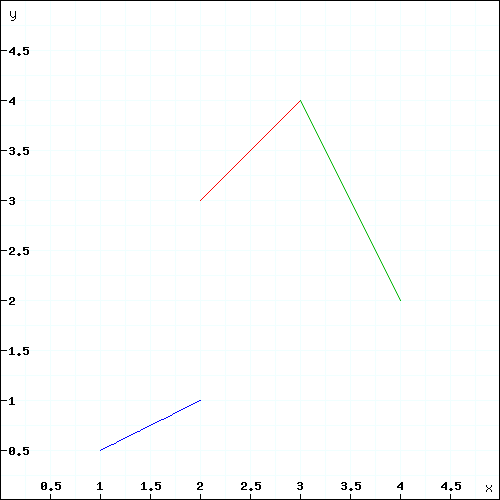
\includegraphics[width=\textwidth,height=\textheight,keepaspectratio]{Laserfunktionskurva} \\
  \caption{figure}{Figur ss. En linjär-interpolerad bild utav avståndsavläsningar från lasersensorn.}
  \label{fig:picture}
\end{center}


\begin{center}
  \includegraphics[width=\textwidth,height=\textheight,keepaspectratio]{Lasersensor} \\
  \caption{figure}{Figur sss. Ett fall där laseravståndsgrafen kommer inntehålla en diskontinuitet.}
  \label{fig:picture}
\end{center}


\begin{center}
  \includegraphics[width=\textwidth,height=\textheight,keepaspectratio]{Lasersensor2} \\
  \caption{figure}{Figur sss. Ett fall där laseravståndsgrafen kommer inntehålla ett lokalt maximum.}
  \label{fig:picture}
\end{center}

Bild på hur kartan sparas

\section{Styrenhet}
Text och blockschema

\section{Sensorenhet}
Text och blockschema
Bild på laser

\section{Mjukvaruklient}
Text och skiss på GUI

\end{document}
